\documentclass[conference]{IEEEtran}
\IEEEoverridecommandlockouts
% The preceding line is only needed to identify funding in the first footnote. If that is unneeded, please comment it out.
\usepackage{cite}
\usepackage{amsmath,amssymb,amsfonts}
\usepackage{algorithmic}
\usepackage{graphicx}
\usepackage{textcomp}
\usepackage{xcolor}
\usepackage{hyperref}
\usepackage{fancyhdr}

\fancypagestyle{firstpage}
{
\renewcommand{\headrulewidth}{0pt}
    \fancyhead{}
    \fancyfoot[C]{}
    \fancyfoot[L]{\textit{Mentor: Professor JayPrakash Lalchandani}}    
    \fancyfoot[R]{ }
}

\urlstyle{same}
\def\BibTeX{{\rm B\kern-.05em{\sc i\kern-.025em b}\kern-.08em
    T\kern-.1667em\lower.7ex\hbox{E}\kern-.125emX}}
\begin{document}

\title{KAPS : \emph{Krishi Avshesh Prabandhan Seva}\\
A Sustainable Rural Waste Management Model
}

\author{\IEEEauthorblockN{Isha Kapoor}
\IEEEauthorblockA{\textit{201701085 - B.Tech ICT}\\
\textit{DA-IICT, Gandhinagar}\\
\textit{201701085@daiict.ac.in}
}
\and
\IEEEauthorblockN{Mahek Rupani}
\IEEEauthorblockA{\textit{201701136 - B.Tech ICT}\\
\textit{DA-IICT, Gandhinagar}\\
\textit{201701136@daiict.ac.in}
}}

\maketitle

\begin{abstract}
The project focuses on providing a potential solution to the issue of rising air pollution because of agricultural residue in India. We have integrated the use of our ICT knowledge to manage our proposed business model. The web application is called Krishi Avashesh Prabandhan Seva (KAPS), a digital portal to manage functionalities of all stakeholders. Scalability of the model in real-life scenario is also explained.\\
\end{abstract}
\begin{IEEEkeywords}
collection, database, schema, user registration, request addition, full stack development
\end{IEEEkeywords}
\section{Introduction}

Crop residue burning is a global phenomena and India is a leading contributor to the burning issue. Harvesting various crops generates large volume of residue. An estimated 500 million tonnes of crop residues are generated annually in India. Emissions from burning biomass leads to significant increase in carbon monoxide, carbon dioxide in the atmosphere, further aggravating the issue of air pollution\cite{b1}. This is illustrated in Figure~\ref{fig:1} for the states in North India. Agricultural residue which is not burned but remains unprocessed in the field leads to methane emission, yet another contributor to global warming. In India, there is no provision for rural waste management, whereas a lot of focus is on urban waste management. The gap between rural and urban waste management policies is shown in Figure~\ref{fig:2}. A series of initiatives have been taken by the Government of India to control this growing issue like providing subsidies to farmers for purchasing agri machinery to process residue. Many private companies have also shown interest in alleviating this problem. \\
But there is no significant relief mainly because of 2 reasons. The first one being,to purchase the subsidised machinery farmers need to spend money on their own apart from the 80 percent subsidy.The other reason is a lack of a singular-nation wide platform to solve this issue. \\
\\
We have tried to achieve a Public Private Platform model through KAPS. There are mainly 3 users types: Collection Centres set up by the government, Farmers and Private Companies that can utilize the residue. The web application functions as a portal for the 3 users where in; a farmer can request for a nearby collection centre to pickup the residue, a collection centre can process that residue so that it can be stored and a private company that can buy the available waste from the residue catalog. KAPS performs a function of an e-commerce website where the farmer is a vendor/manufacturer and the private company is the consumer. The collection centre manages the orders, processes the incoming waste and performs the biomass characterisation for it. The farmer receives and the private company pays a fixed amount of money for a kilogram of waste. \\
\\
KAPS enables the farmers to generate additional revenue while encouraging private companies to use sustainable energy generation techniques and make green products. The network of collection Centres would provide a uniform platform and act as a one time investment for the country. With a urban waste management system already in place, KAPS would be the rural waste management system for our country.  
\begin{figure}[htbp]
\centerline{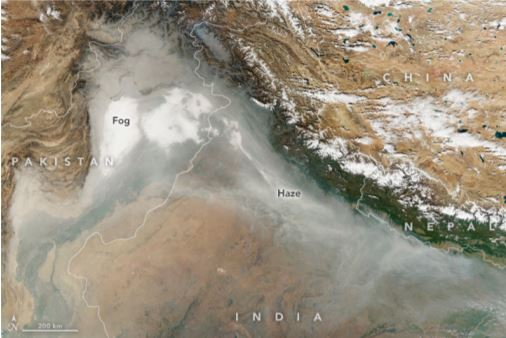
\includegraphics[width=0.5\textwidth,  height=5cm , ,keepaspectratio]{Capture.JPG}}
\caption{NASA Earth Observatory image of fog and haze distribution over the Northern States of
India after Parali burning in November 2017 }
\label{fig:1}
\end{figure}
\begin{figure}[htbp]
\centerline{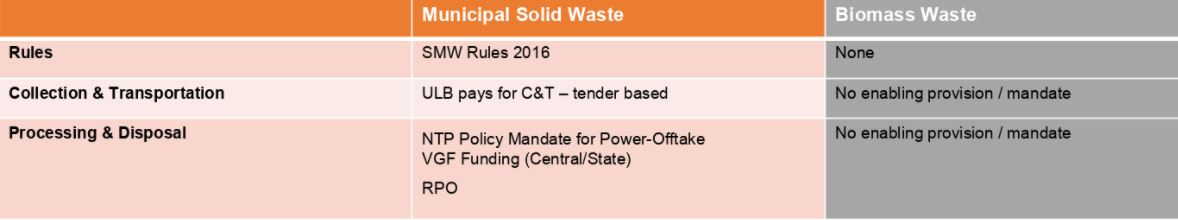
\includegraphics[width=0.5\textwidth,  height=15cm , ,keepaspectratio]{Capture1.JPG}}
\caption{Comparison between Urban and Rural Waste Mnagement Policies in India}
\label{fig:2}
\end{figure}\\
\thispagestyle{firstpage}

\section{Pre-Project Field Work}
To understand if our vision was viable and gather basic understandings of policies already in place, we approached Abellon CleanEnergy Ltd\cite{b2}. Abellon is a pioneer in the Waste-to-Energy sector in India, with a vision to contribute to nation building through sustainable energy solutions for Power, Heat and Transport. \\
We had meetings to set up the base of the project. The officials at Abellon enlighted us about the lack of a rural waste management system in India, and encouraged us to venture into this domain. They themselves have a rural waste to energy chain with only a few farms in Gujarat but due to lack of a systematic framework and book-keeping, they often encounter legal issues with farmers. \\
They provided us with their adopted model and we discussed the loopholes in it, which made us realise the need of a digital solution for the same, thus leading us to build KAPS.
\section{User Stories}
As part of the project, we identified the four stakeholders: Farmers, Collection Centre, Private companies and Admin. We then developed the user stories for each stake holder. They can be broadly divided as follows: \\
A basic login, registration, logout and profile viewing functionality was required for all stakeholders.
\begin{itemize}
\item Farmer Requirements
   \begin{itemize}
       \item As a farmer the primary requirement was to be able to request waste pick-up according to the crop harvesting date 
       \item A waste residue catalogue was required so that farmer could identify the residues for each crop 
       \item A notification system for receiving timely updates so that farmer can be on the farm was needed 
   \end{itemize}
\item Private Company Requirements
\begin{itemize}
    \item Each private company needed to enter their product details for which raw materials will be used 
    \item A order placing system to place order and view the availability of ready waste at different collection centre to choose from was a required functionality 
\end{itemize}
\item Collection Centre Requirements 
\begin{itemize}
    \item Each collection centre required a robust order tracking system to approve, enter waste details and close order in an efficient manner 
    \item A portal to enter biomass characterization details of each residue was required 
    \item An automatic calculation of incoming waste and ready waste was needed after being able to update the processing waste 
\end{itemize}
\item Admin Requirements
\begin{itemize}
    \item A complete visualization to manage and remove users 
    \item A functionality to set prices for waste as per the market value was required in place to keep the system up to date with real-world prices
\end{itemize}
\end{itemize}

\section{UML Design}
\subsection{Class Diagram}
The Figure~\ref{fig:001} shows the class diagram of the system.
\begin{figure}[htbp]
\centerline{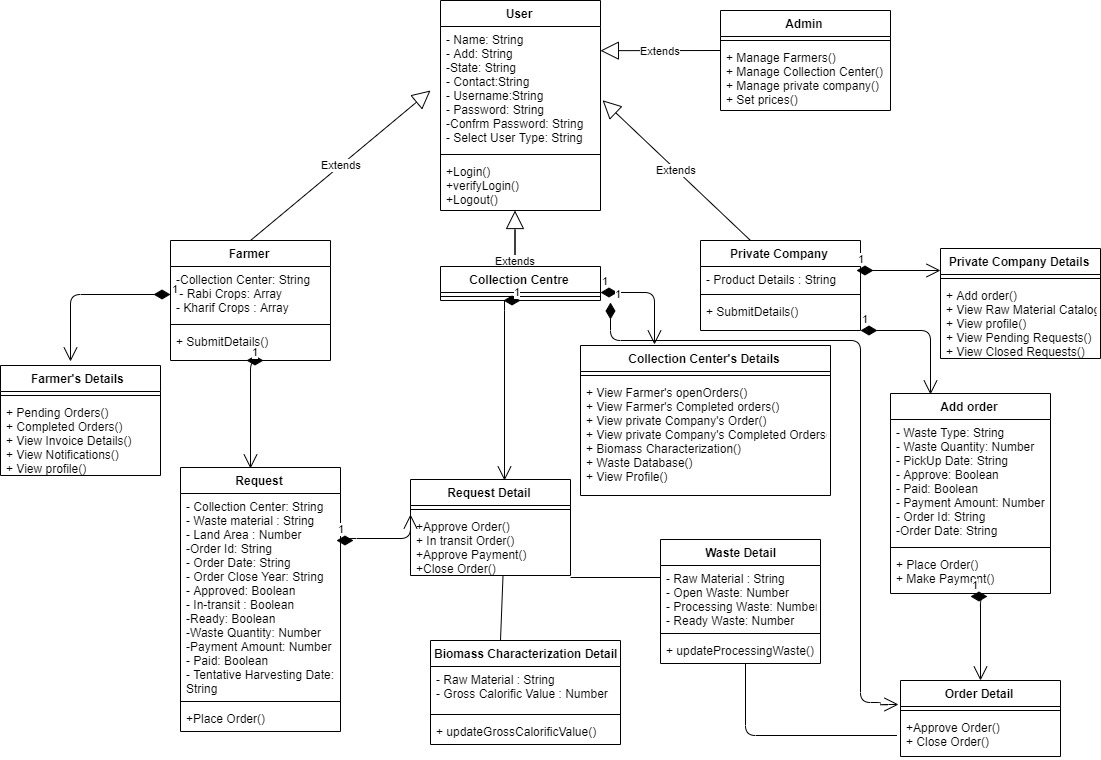
\includegraphics[width=0.5\textwidth ,keepaspectratio]{Class1.jpg}}
\caption{Class Diagram}
\label{fig:001}
\end{figure}
\subsection{Sequence Diagrams}
This section shows Figure \ref{fig:a} , Figure ~\ref{fig:c} , and Figure ~\ref{fig:b} depicting the sequence diagrams.
\begin{figure}[htbp]
\centerline{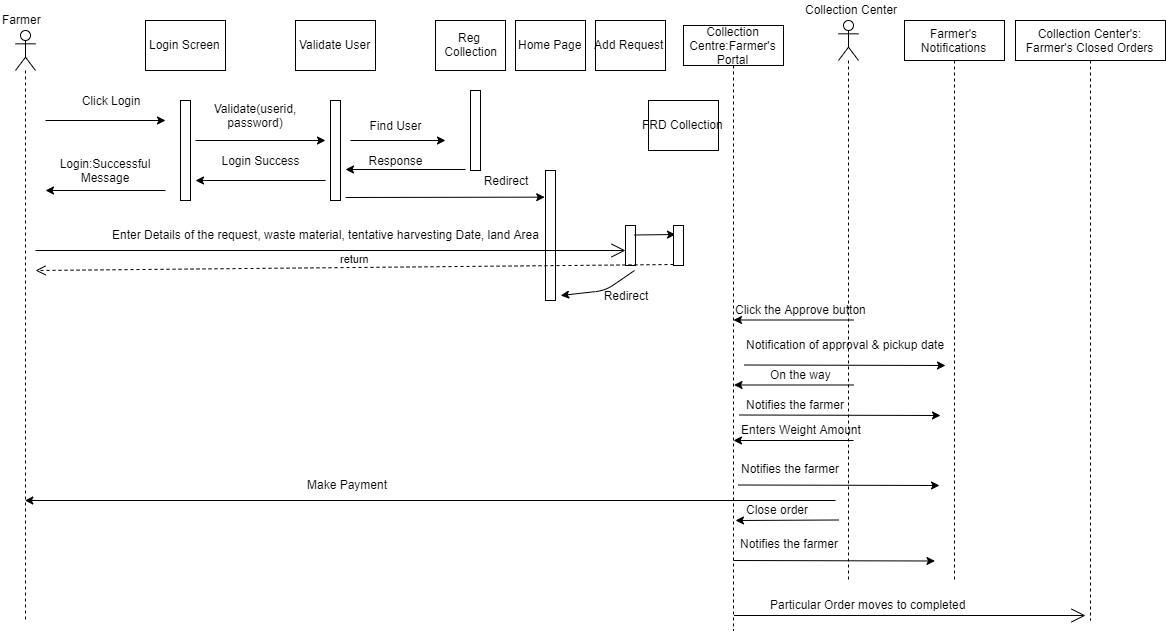
\includegraphics[width=0.5\textwidth,  height=10cm , ,keepaspectratio]{FF.png}}
\caption{Sequence diagram indicating the steps followed by a farmer for requesting pickup and how the collection center acts on the record. This record gets stored in Farmer's Request Details Collection. }
\label{fig:a}
\end{figure}
\begin{figure}[htbp]
\centerline{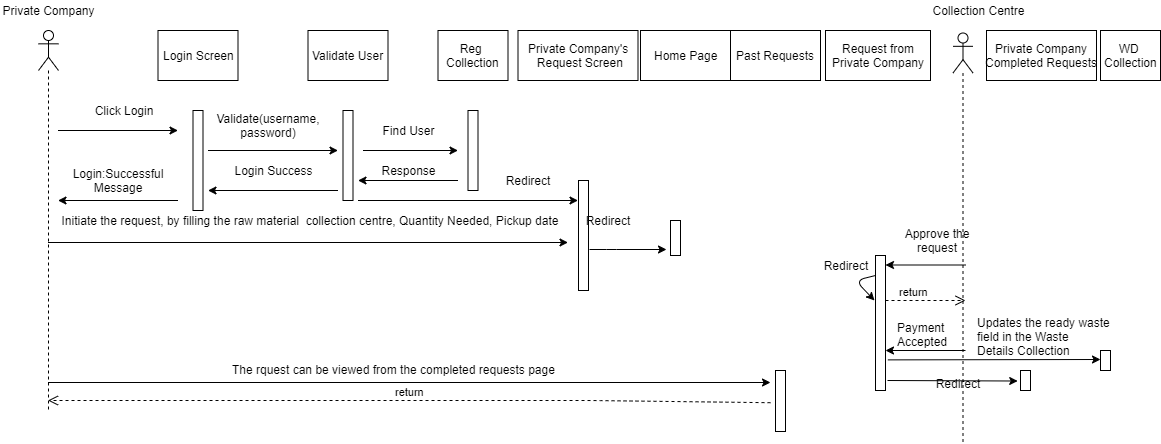
\includegraphics[width=0.5\textwidth,  height=10cm , ,keepaspectratio]{PCF.png}}
\caption{Sequence diagram indicating the steps followed by a private company to book a order and how the collection center acts on the order. This order gets stored in Private Company Order Details Collection. }
\label{fig:c}
\end{figure}
\begin{figure}[htbp]
\centerline{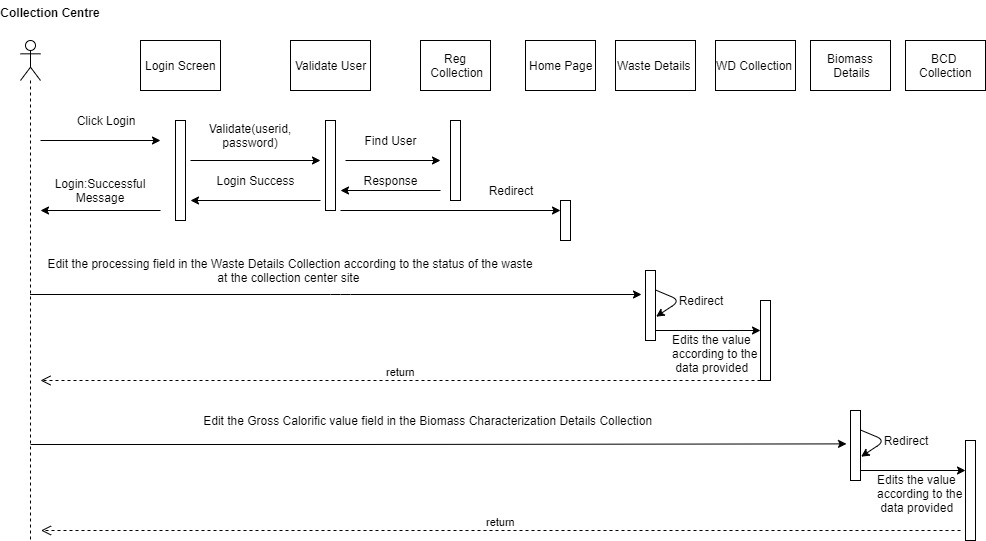
\includegraphics[width=0.5\textwidth,  height=10cm , ,keepaspectratio]{CCF.jpg}}
\caption{Sequence diagram indicating the steps followed by a collection center to update the Waste Details Collection and Biomass Characterization Details Collection. }
\label{fig:b}
\end{figure}

\section{System Requirements}

 
\subsection{Tech Stack}
\begin{itemize}
    \item Back end run time environment: \href{https://nodejs.org/en/}{Node.js\cite{b3}}
    \item Server framework: \href{https://expressjs.com/}{Express.js\cite{b4}}
    \item Front End: \href{https://www.w3schools.com/html/default.asp}{HTML\cite{b5}}, \href{https://www.w3schools.com/css/default.asp}{CSS\cite{b6}}, \href{https://www.javascript.com/}{JavaScript\cite{b7}}
    \item Database: \href{https://www.mongodb.com/}{MongoDB\cite{b8}}
    \item Templating Language: \href{https://ejs.co/}{EJS\cite{b9}}
\end{itemize}
\subsection{UI/UX Design}
The tool used to design the visual aspect of the project is Figma. It makes the developer handoff process significantly smoother.
\section{Solution Design}
\subsection{Setup}
The initial setup of the system is done using Github . The installations of several packages and libraries were required such as node, mongodb,  bcryptjs, cookie-parser, dotenv, ejs, express, jsonwebtoken, moment, mongoose, and nodemon.\\
\subsection{Overview Of the Technologies Used}
\begin{itemize}
    \item Node is a JavaScript environment that allows you to run server-side JavaScript.
    \item Express.js is a Node js web application server framework. It responds to the requests with route support so that the responses are written to specific URLs.
    \item HTML is a standard markup language for structuring Web Page.
    \item CSS determines how the HTML elements will look like.
    \item Javascript is the scripting language which is used to create dynamic content. 
    \item MongoDB is a database that stores the data as documents. These documents resemble json like structure. JSON documents created in the front end can be sent to the Express.js server, where they can be processed and  stored directly in MongoDB for later retrieval.
    \item Bcrypt provides password hashing methods. bcrypt.hash() takes in the password that user wants to set and the salt rounds as input. Salt rounds is a synonym used for the cost factor to calculate the hash. It returns the hashed string as the output which is stored in the database in the password field. bcrypt.compare() is used for comparing the stored password in the database and the password that user inputs during login.
    \item jsonwebtoken it takes in the input of the user ID and the secret key and generates a token which would be saved in the database to mark the user logged in. When the user registers or login this token is created.
    \item Since our system uses cookies based authentication system the cookie-parser sets the cookie with the generated token.
    \item Dotenv is a zero-dependency module that loads environment variables from a .env file into process.env. This file contain our hidden information about the secret key, the database URL, and the admin credentials.
    \item EJS templates contain HTML, along with special ejs tags which embed a Javascript expression whose return value will be added to the template when compiled. 
    \item Moment is a javascript date library that helps create, manipulate, and format dates without extending the Date prototype. It helped us to store the date in a string format.
    \item Mongoose is basically a package that serves as a mediator between the NodeJS application and MongoDB server. Mongoose schema as a blueprint for defining the structure of a Mongoose model that maps directly to a MongoDB collection.
    \item nodemon monitors for any changes in the source and automatically restarts the server.
    \item Anychart is a javascript charting library which helped in data visualization. 
\end{itemize}
\subsection{Run}
As of now, one needs to navigate to the root directory of the project and type the command [npm i] this installs all the dependencies listed in the package.json. After successfully installing the above packages, hit  [npm run dev]  on the command prompt/terminal. Once the setup is done the user can reach this part through the link: \( <localhost:3000 >/ \). The user will be greeted with the home screen as shown in Figure~\ref{fig:3}.
\begin{figure}[htbp]
\centerline{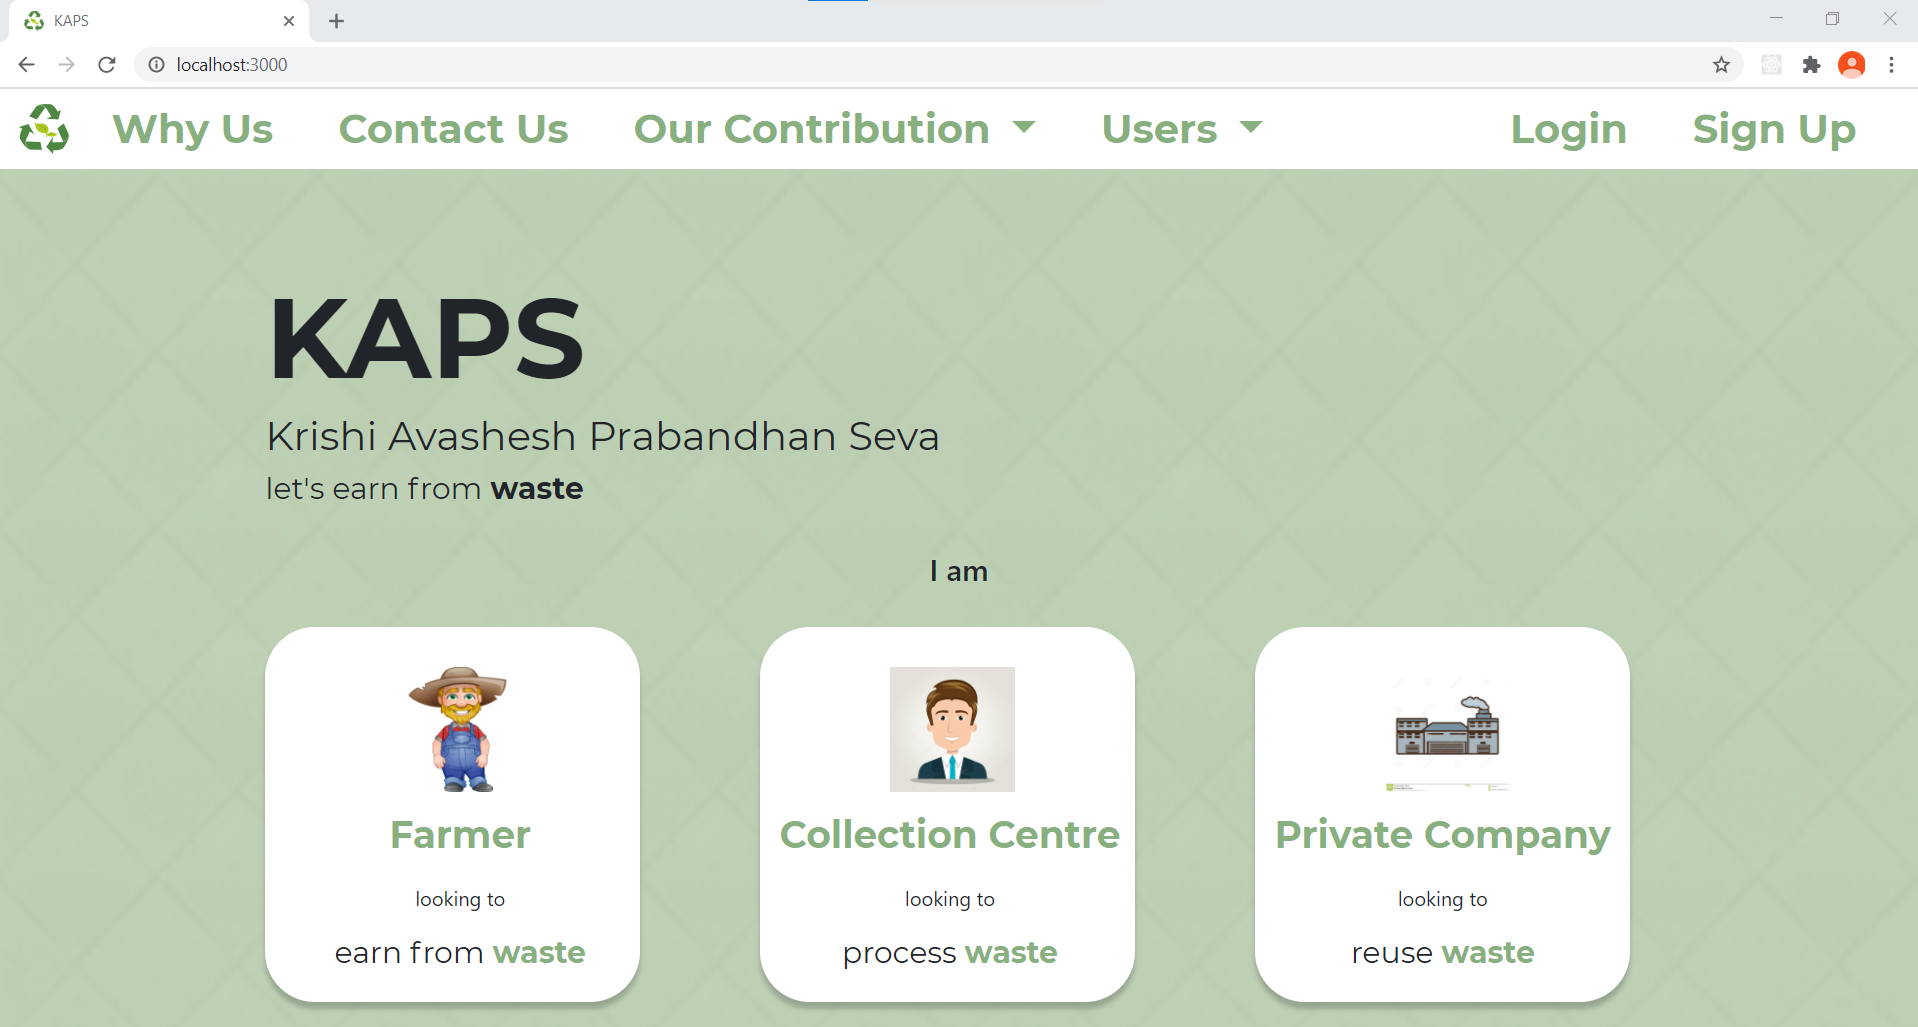
\includegraphics[width=0.5\textwidth , height =4.7cm ]{Home.png}}
\caption{The Home Page}
\label{fig:3}
\end{figure}
\subsection{Database Schemas}
As mentioned earlier, all the database collections are stored using MongoDB. As soon as a record is created in any collection a unique \_id with the type ObjectID is also created as shown in Figure~\ref{fig:4}. The Refid field mentioned in the Schema is the unique \_id of the user who initiates the request. For further details about the Database Schemas refer Appendix A.
\begin{figure}[htbp]
\centerline{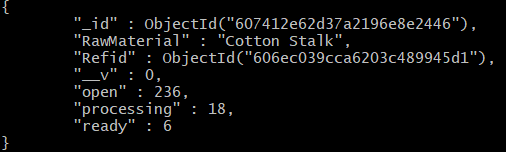
\includegraphics[width=0.5\textwidth , height=2.2cm]{Data.png}}
\caption{Example of \_id creation}
\label{fig:4}
\end{figure}


\section{System Workflow}
As shown in the Figure~\ref{fig:5}, when the user registers it is redirected to the specific route according to the user role, and the data is saved in the Reg collection(See Appendix A and B).  While Registering to the system, if the name and the username fields are unique and the password and confirm password fields match then only the details are saved in the Reg Collection.  If the user is a farmer or a private company and no collection center is registered in that state then the user won't be able to make an account. The above procedure is checked via the Reg collection's fields Select User Type and State (See Appendix A). If the user is a Farmer is then allowed to submit the crop details and the collection center's details and this data is then saved into FCD collection and is then taken to its home page. If the user is a private company then it has to fill in the details of the product that it makes and is then navigated to its home page. And if the user is of type Collection Centre it is directed to its home page. If the user is a farmer or a private company and it tries to log in without filling in the additional details i.e the details of FCD Schema and PCPD Schema respectively, then their account is permanently deleted.\\
\begin{figure}[htbp]
\centerline{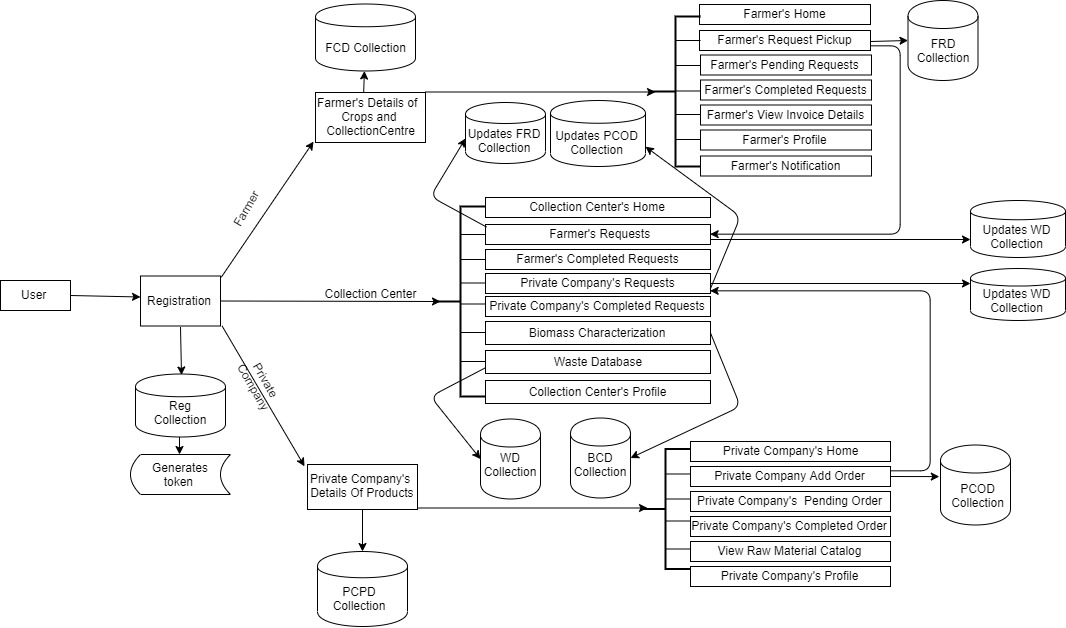
\includegraphics[width=0.5\textwidth,  height=11cm , ,keepaspectratio]{Layout1.jpg}}
\caption{Layout of the Solution}
\label{fig:5}
\end{figure}
\begin{itemize}
\item The Farmer sees the type of residue based on the crops that they grow on the Farmer's Request pickup page. For example, a user fills in the details of crops as cotton and Rice. So the user sees the raw materials as shown in the Figure~\ref{fig:16}. The front-end service accepts the farmer’s waste pickup request to send it to the designated collection center. The first order of business is to generate a unique order ID and set up a record in FRD collection that contains the detail of the farmer’s request and also states that the approval is pending. This record will be used to communicate with the farmer about the status of the request. The farmer can view this record on the Farmer's pending request page.
\begin{figure}[htbp]
\centerline{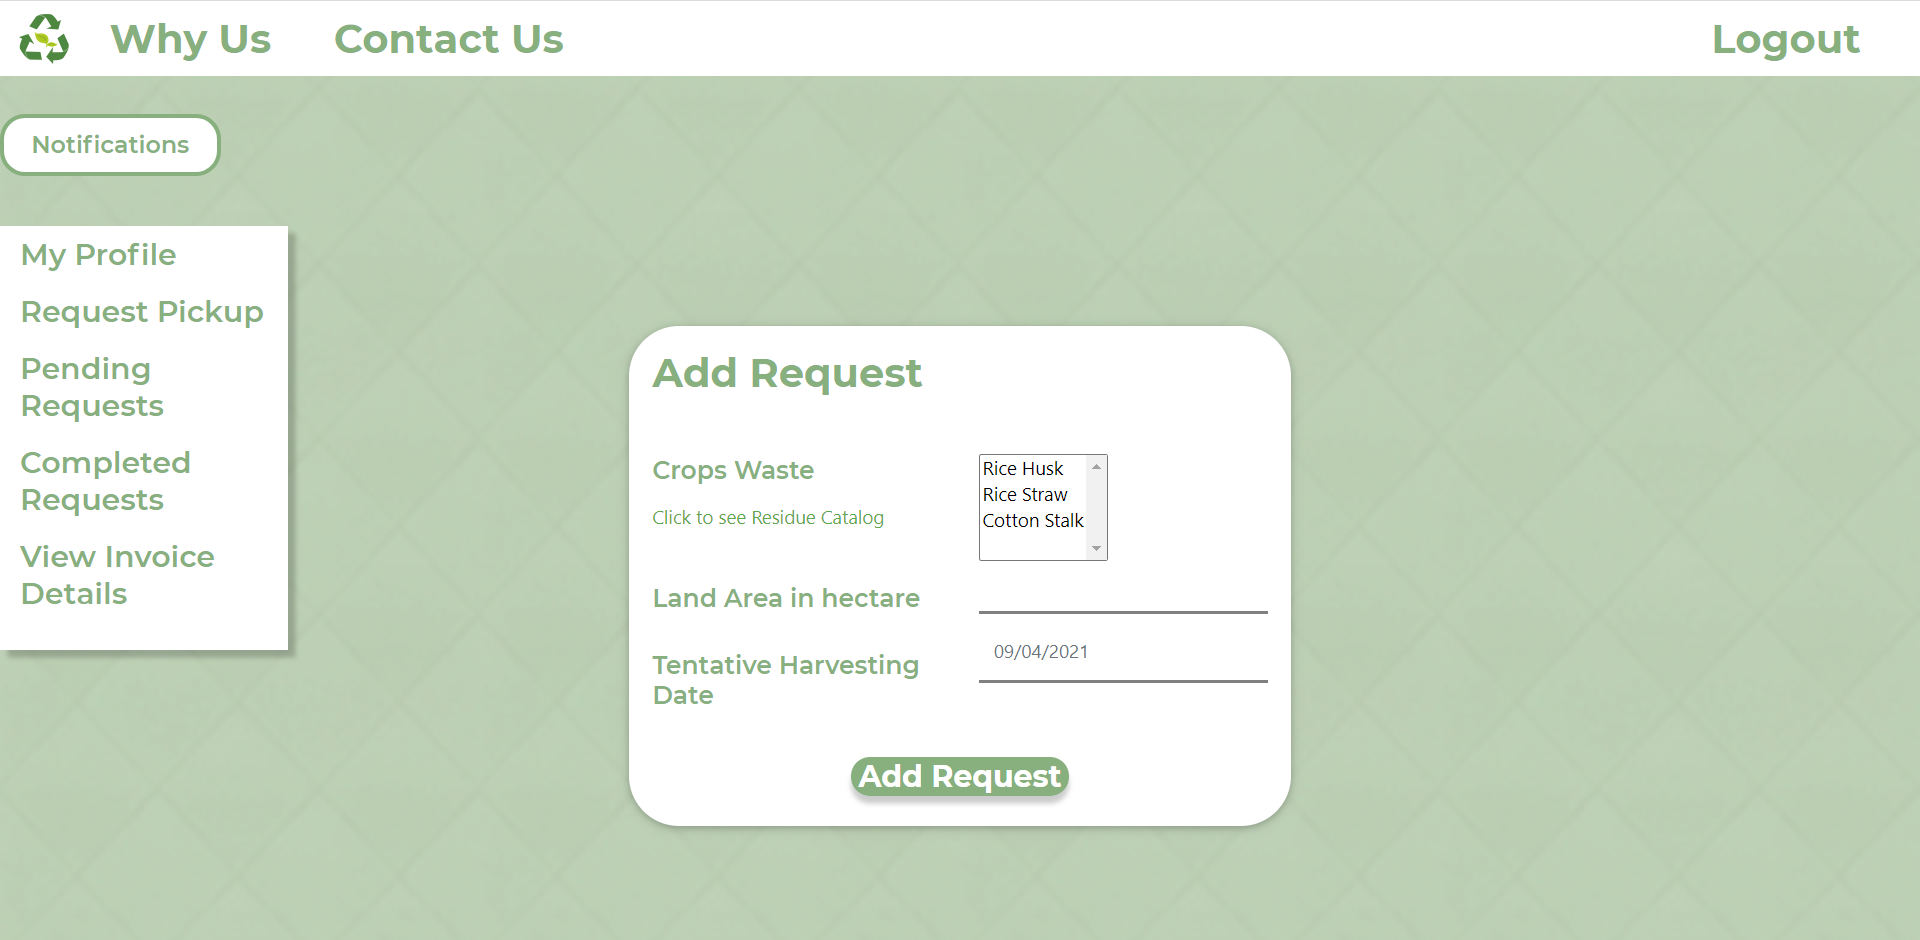
\includegraphics[width=0.5\textwidth,  height=12cm , ,keepaspectratio]{Example1.png}}
\caption{Raw Material Detail According to Crops Registered}
\label{fig:16}
\end{figure}
\item On receiving the request from the Farmer, the collection center sees the record on the Farmer's Request page where it provides the status of the request (approved/in transit/paid) and the pickup date to the farmer. As soon as these details are furnished the FRD collection is updated and the Farmer is notified. The farmer can view these details on the Farmer's view invoice details page and the notification page. 
\item When the waste measurement is completed at the collection center's site, the front end service then accepts the waste amount and sends it to the Farmer. Also, the FRD collection and the open waste field in the WD collection get updated.
\item As soon as the payment is completed and the FRD collection is updated that record is then moved to the completed request status for both the stakeholders involved. 
\item The collection center can update the processing field in the WD Collection according to the waste being processed by the machinery at the site. The update in the processing field either results in a decrease in the open waste field or an increase in the ready waste field in the WD collection.
\item The Private Company has the complete right to view the available raw materials, its quantity, and their biomass characterization at the collection center of their respective states using the details the WD collection and the BCD Collection. When it initiates the request to the collection center, if the ordered raw material is not available at the collection center or is available in less quantity which is checked via the WD collection then the order can not be placed. if all the above conditions are satisfied then a unique ID is generated and the request details are stored in the PCOD Collection.
\item As the collection center sees the request of the Private Company on the Private Company's Request page it acts upon the request and provides the status to the private company and the PCOD Collection is updated.
\item The private company can then view the status on the Private Company's pending order details page.
\item On receiving the payment, the collection center marks the order as completed by updating the PCOD Collection. According to the raw material and the quantity collected by the private company the ready waste field value decreases in the WD Collection. Both the stakeholders involved can view this record on the completed requests page.
\item The Admin has the right to view all the users and can also permanently suspend the user account by deleting it from the designated collections. 
\item The Admin has the right to change the price per kg of the raw materials at which the private company buys it and also the price which collection center pays the farmer for 1 Kg waste which is done from the WP Collection.
\end{itemize}
\section{Architecture}
Figure~\ref{fig:6} shows the architecture of KAPS.
\begin{figure}[htbp]
\centerline{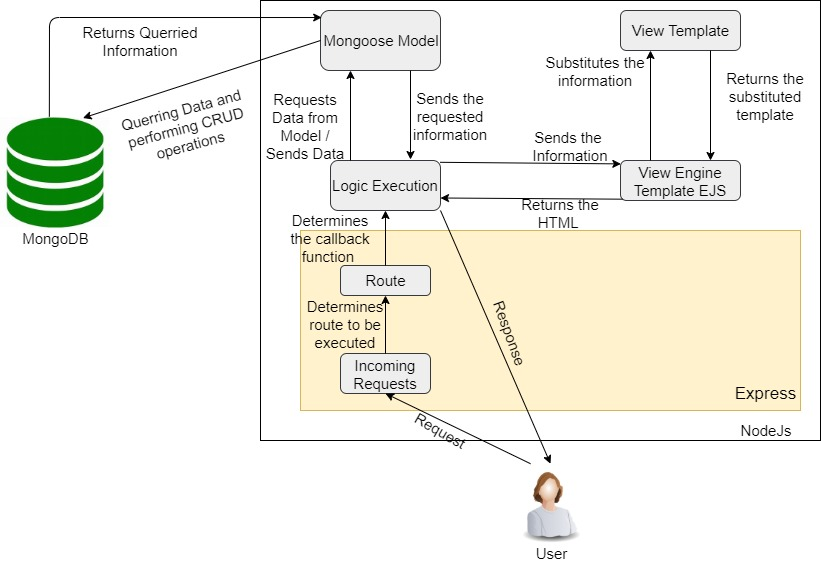
\includegraphics[width=0.5\textwidth,  height=12cm , ,keepaspectratio]{Arch .jpg}}
\caption{Architecture of the Solution}
\label{fig:6}
\end{figure}
\begin{itemize}
    \item Incoming Requests: This process all the requests coming from the user. It also determines which Express middleware route would be executed.
    \item Route: It is a Express middleware HTTP request path. For example:
    \( app.get("/whyus" ,callback) \). Here, the HTTP GET method on the path "/whyus" is defined to be a route handled by the callback function of the logic executor.
    \item Logic Execution: This recieves the requests and processes the requested data and retrieve the information needed from the Mongoose model. After its execution,the data is passed to the view template engine(ejs) for rendering to the client.
    \item Mongoose Model: It provides a mapping from a model to the raw data.
    \item View Template Engine EJS: It takes the data from the Logic Execution module and substitutes it into the view template.
    \item View Template: It returns the response for a particular request. It is a HTML file with markup for variable substitution. For example the username of the user is depicted by \(<\%=records.username \%>\).
\end{itemize}

\section{Results and Analysis}
Our website serves as a e-commerce portal for buying and selling of agricultural residue and as a portal for tracking all the orders by the collection centre.\\ We tried to take our project one step further by analysing the impact of the model in one year. We asked different people to act as demo users and feed in order pick-up and drop of requests from January 2021. On completing those requests, KAPS computed 4 parameters which are: Total Waste Collected(Figure~\ref{fig:z}), Revenue Earned(Figure~\ref{fig:y}), Sustainable Products Made(Figure~\ref{fig:x}),Reduction of Carbon Emission. Our website has a feature that generates pictorial representation of these parameters, so that all the users can see the large scale impact of KAPS. 
\begin{figure}[htbp]
\centerline{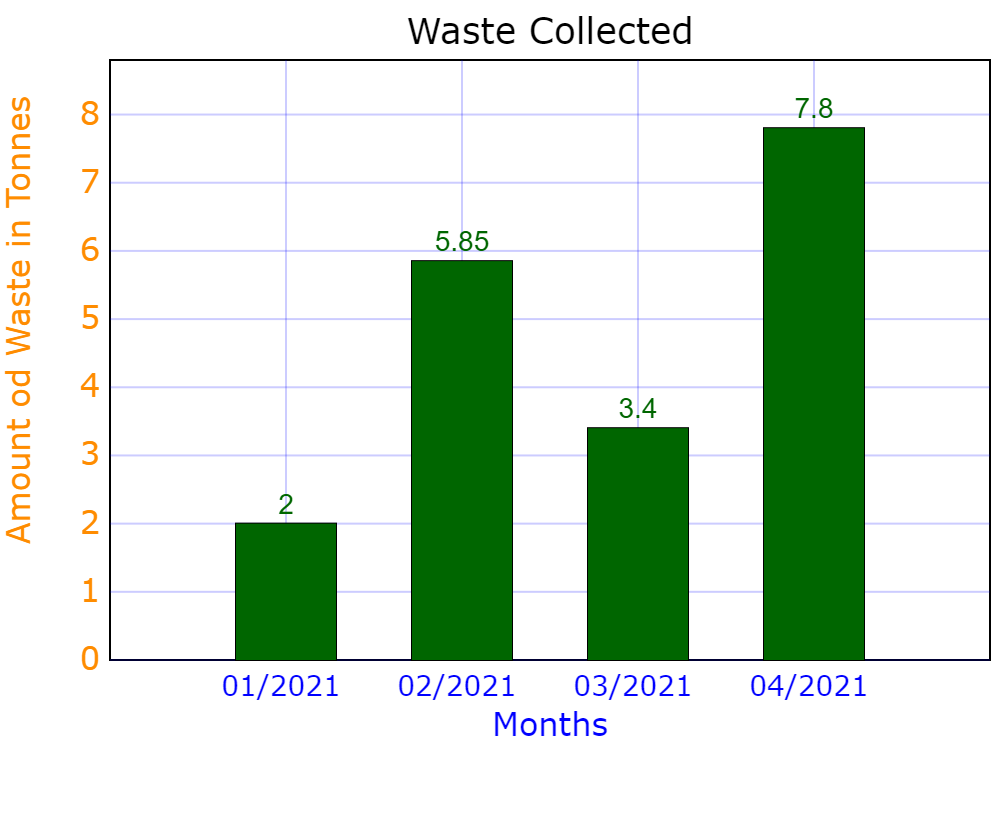
\includegraphics[width=0.5\textwidth,  height=6cm ,keepaspectratio]{WasteC1.png}}
\caption{Amount of Waste Collected From Farmer Per Month}
\label{fig:z}
\end{figure}
\begin{itemize}
    \item The total amount of waste collected from farmers (demo requests) in 4 months, from January 2021 to April 2021 is: \\
    2 + 5.85 + 3.4 + 7.8 = 19.05 Tonnes or 19050 kg.
    \item Each kilogram of residue on burning releases : 1.2 kg of Carbon Dioxide in the atmosphere.
    \item Potential Carbon emission of the above waste is : 19050*1.2 = 22,860 kg
    \item This is just a drop in the ocean compared to the total amount of carbon emission we can curb by adopting this model. India generates around 500 Mt of agri-waste out of which 140 Mt is burnt. 
    \item The potential scope of reduction in carbon emission in one year is : 140*1000,000*1000*1.2 = 168 Billion Kg of Carbon Cut.
\end{itemize}
\begin{figure}[htbp]
\centerline{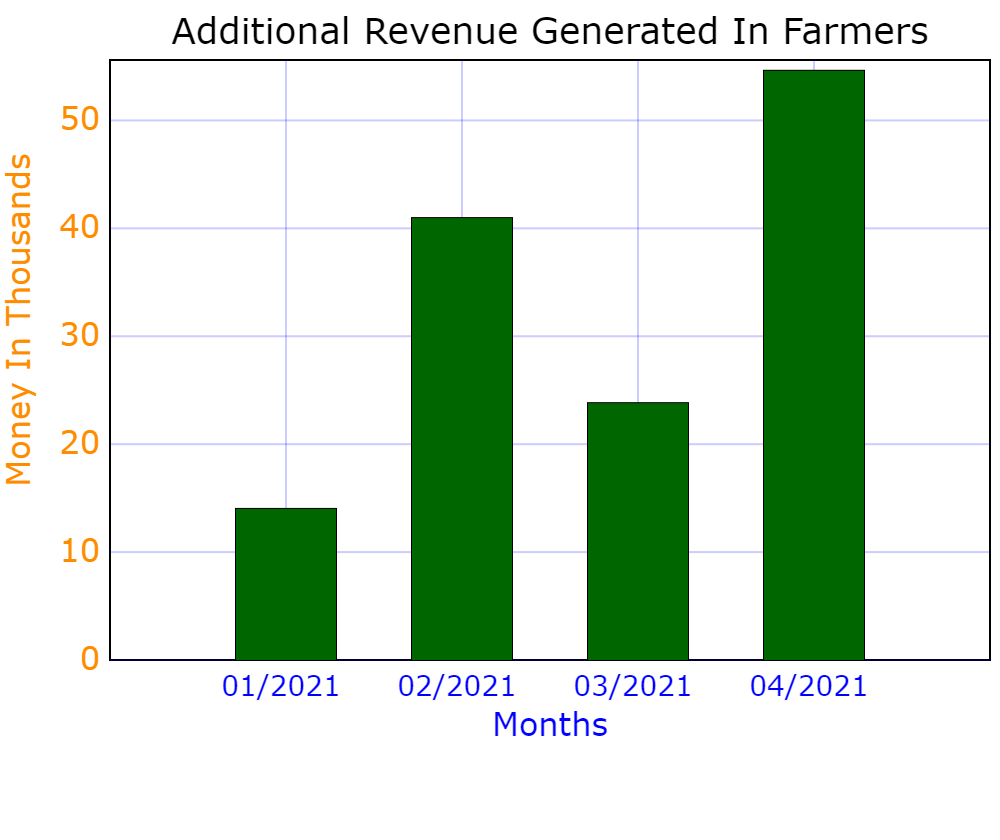
\includegraphics[width=0.5\textwidth,  height=6cm ,keepaspectratio]{Revenue1.png}}
\caption{Revenue Earned by Farmer per Month}
\label{fig:y}
\end{figure}
\begin{figure}[htbp]
\centerline{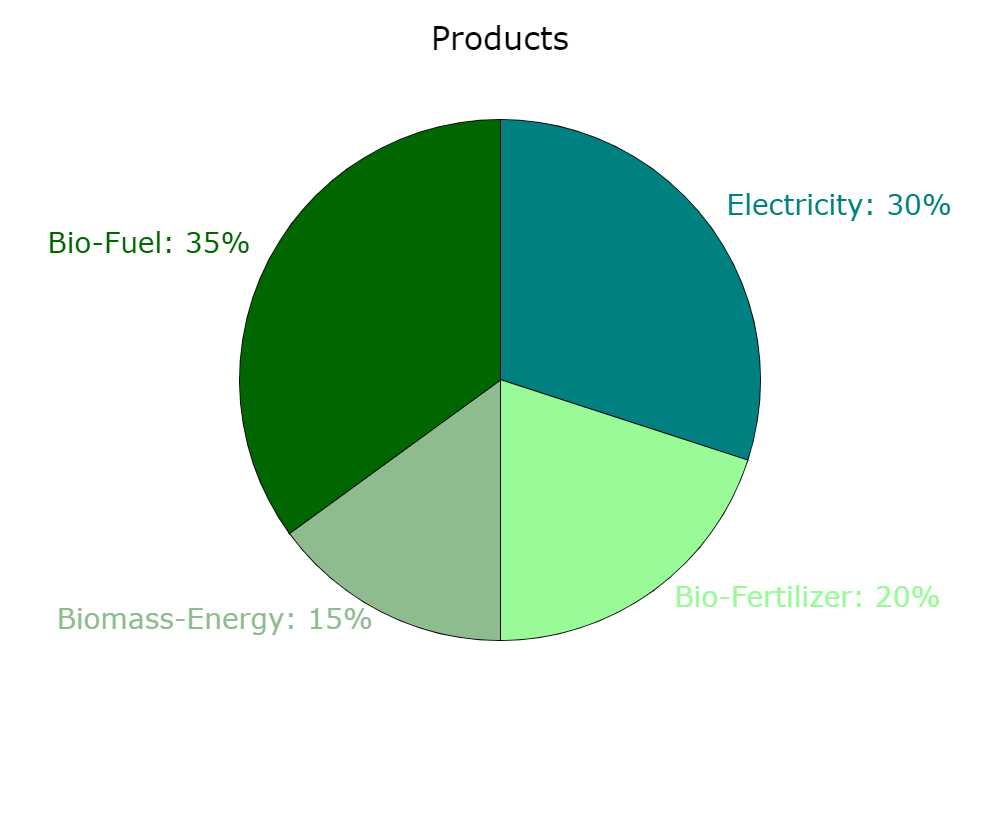
\includegraphics[width=0.5\textwidth,  height=6cm ,keepaspectratio]{Products1.png}}
\caption{Registered products by Private Companies}
\label{fig:x}
\end{figure}
\section{Post-Project Field Work}
After completion of the website, we met with Abellon officials to show the demo and gain feedback from them. They tested the working of the website and reverted back with positive comments. Mr. Pankaj Patel, the president of the company appreciated our initiative as we realized a problem and effectively designed a solution to process agriculture residue. \\
We learnt about one essential component that could be added to our project. In India, there are zamindars that rent out their lands to farmers for growing their crops. This is called the owner and grower system. So it is possible that a zamindar rents a piece of land to one farmer in a particular harvest season and the tenant changes in the next season. Currently KAPS registers farmers but does not take into account of their ownership status. Adding this feature would make KAPS more coherent with the farming ecosystem in India. We plan on incorporating this feature in the future, the same has been added to the future scope section as well.
\section{Scalability of Business Model}
A decentralized model will prove to be efficient in this case, as it would be easier to set up a PAN India network of farmers and private companies. Setting up a new collection centre is easier in this model, making it replicable. We have taken inspiration from the 'Amazon' retail supply chain management. \\
\begin{itemize}
    \item To understand the scalability of the project we assessed India as a whole, to propose location of collection centres. 
\begin{itemize}
    \item Area of India: 3287000 sq km 
    \item Land Utilized for Agriculture: 1597000 sq km (48\%)
    \item Proposed Locations of Collection Centres: According to our research, each collection centre should be located in 15-20 km radius from the agricultural farms. This is mainly because of two reasons: 
    \begin{itemize} 
        \item The distance within this range is sustainable for collection centres to travel and pickup farm residues 
        \item There are some farmers with tractors, who themselves want to drop off the waste can reach the collection centre with this range 
    \end{itemize}
    According to these calculations, and subtracting out the urban developed land, we have pin-pointed suitable collection centre locations in India in Figure ~\ref{fig:7}. 
    \begin{figure}[htbp]
\centerline{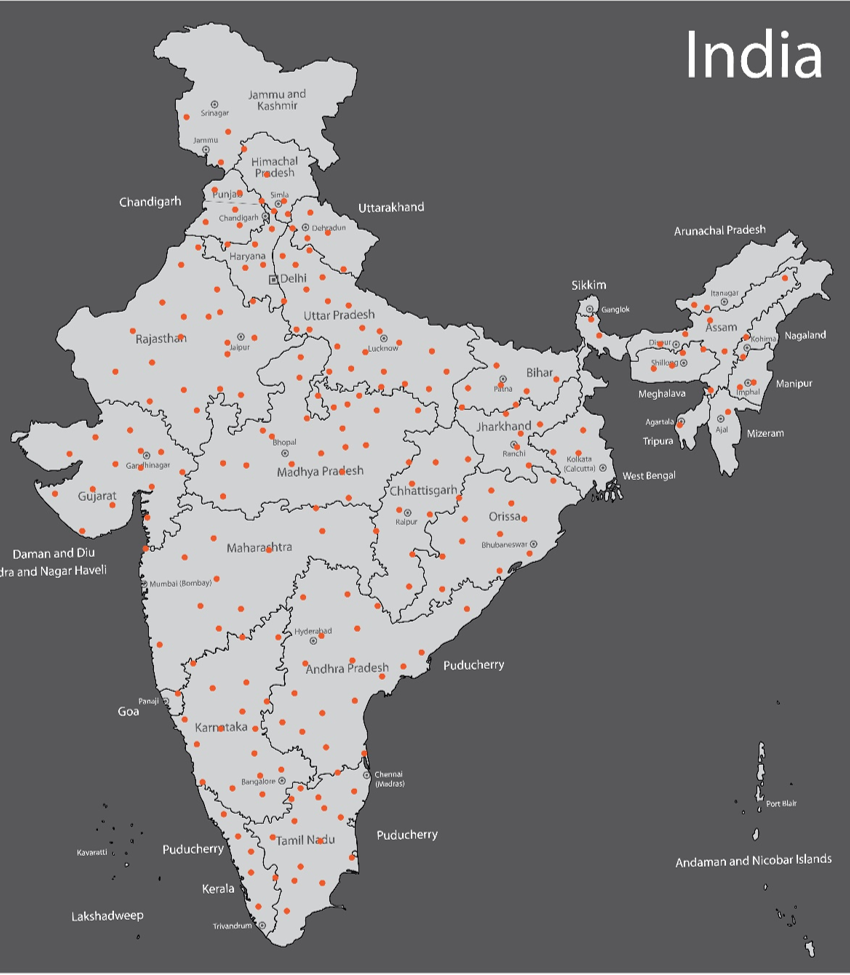
\includegraphics[width=0.5\textwidth,  height=10cm , ,keepaspectratio]{Picture1.png}}
\caption{Collection Centre Locations}
\label{fig:7}
\end{figure}
\end{itemize}
\item Cost for Collection Centre includes the initial cost of constructing the Collection Centre. This cost will vary depending on the state and size of the centre.The secondary costs or recurring costs will include salaries, maintenance and insurance costs. \\
 The size of collection centre will depend on the amount of incoming waste, for example, states like Punjab, Haryana, Gujarat will have larger sites than other states. \\
 The different collection centres based on capacity are: 
\begin{itemize}
    \item Small sized  : Capacity of 50, 100, 200, 250 Mt
    \item Medium sized : Capacity of 500, 1000, 2000 Mt
    \item Large sized : Capacity above 2000 Mt
\end{itemize}
The actual costs and returns will have to be taken on a case by case basis considering the specific requirements of projects. 
\item The second important component of the model is transportation of waste. If farmers have their own tractors and it is convenient for them to drop off the waste, it would add value addition to the assets that the farmer already has. Similarly, the private company could also send their trucks for order pick-up. \\
Each collection centre will also require trucks(Figure ~\ref{fig:8}) for loading/unloading waste from farmer fields and delivering to private companies. The main pickup trucks for garbage collection are as follows: 
\begin{itemize}
    \item Pickup trucks for waste collection: 
    \begin{itemize}

            \item Compactor Trucks : capable of collecting garbage / organic waste, compacting  the same and transporting it to designated landfills/disposal site
            \item Bulk Refuse carrier : a garbage collecting and transporting vehicle
            \end{itemize}
    \begin{figure}[htbp]
\centerline{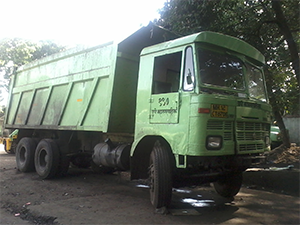
\includegraphics[width=0.5\textwidth,  height=5cm , ,keepaspectratio]{B-R-C.png}}
\caption{Trucks for Waste Collection}
\label{fig:8}
\end{figure}
\end{itemize}
\item Machinery for residue processing: 
    The residue collected occupies a lot of volume as compared to its weight. Further, keeping the waste in open is not suitable as it can catch fire or start degrading. Therefore, various machines are required at the collection centre to process the waste for the use of private companies. 
    \begin{itemize}
        \item Waste Weighing Machine : This is industry grade weighing machine as the payment are solely based on the weight of residue collected or sold 
        \item Fodder block machine : The fodder block(Figure~\ref{fig:9}) or the feed block making machines compress the dried crop residues into blocks that can be stored and later fed to the cattle during the lean season.
         \begin{figure}[htbp]
         \centerline{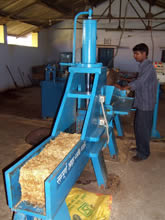
\includegraphics[width=0.5\textwidth,  height=6cm , ,keepaspectratio]{unnamed.jpg}}
         \caption{Fodder Block Machine}
         \label{fig:9}
         \end{figure}
\item Agricultural Waste Shredder and Chipper: Waste can be converted to valuable mulch or high quality compost material
\end{itemize}
\item Biomass characterisation laboratory set-up: Every crop residue has a specific calorific value. The ideal calorific value of 1 kilogram of average ready waste is around 3800 kilo calories. Biomass characterisation is an essential step to understand the bio-chemical and physical properties of the waste which are required to calculate the calorific value of waste residue.It is required to determine the viability/quality of residue to be used as raw material for private company. Therefore, every collection centre would require a small lab set-up to conduct biomass characterisation.
\end{itemize}
 
\section{Benefits of the System} 
The system has manifold advantages, such as: 
\begin{itemize} 
\item Each kilogram of average ready waste when compared with 1 kg of average Indian coal, releases 1.2 kg of carbon dioxide into the atmosphere. On an average 500 Mt of crop residue is generated yearly in India. While a majority of it is used
for fodder, raw material etc., still there is a huge surplus of 140 Mt out of which 92 Mt is burnt each year. This 140 Mt releases approximately 168 billion kg of CO\(2\) every year. KAPS curbs this inflow of carbon dioxide into the atmosphere. \cite{b10}
\item Our system acts as the "carrot and sticks" approach. The  Farmer who do not burn their waste and instead ask the collection  center to collect the waste gain monetary benefits. 
\item Value addition of assets takes place in our model. Farmers or private companies who have trucks or tractors that have no utilization during the evenings or nights, can use them to transport residue to and from collection centre respectively. 
\item The private companies who are the producer of Biofuel,  Biomass, Electricity, Bio-fertilizers, etc who need these waste  products as their raw materials can also get them easily by the system. 
\item The calorific value of Indian coal is 3500 kcal/kg. Energy production using coal, leads to burning and using fossil fuels which inturn depletes their quantity and harms the environment. Instead, using biomass from farms can generate 3800 kcal/kg, which is higher than coal and protects the environment. 
\item The system is also like "killing two birds with one stone". In this procedure the farmer gets money even from the waste, the greenhouse gas emissions are also reduced by a significant amount, and the production of various green products can be done.
 
\end{itemize}
\section{Testing}
\subsection{Case: Maintenance of the Waste}
The collection center has the responsibility of changing the processed waste. When the collection center provides the waste quantity to the farmer for the specific record the open waste increases by the waste quantity. When a private company orders a raw material, and is approved by the collection center the value of the ready waste decreases by the quantity ordered. When the waste is in the processing state the collection center needs to update the processing field. \\ 
For example, currently, the waste statistics of Wheat Husk are open waste: 7kg, processing waste: 3Kg, ready waste: 2Kg as shown in the figure~\ref{fig:10}.\\ 
        \begin{figure}[htbp]
         \centerline{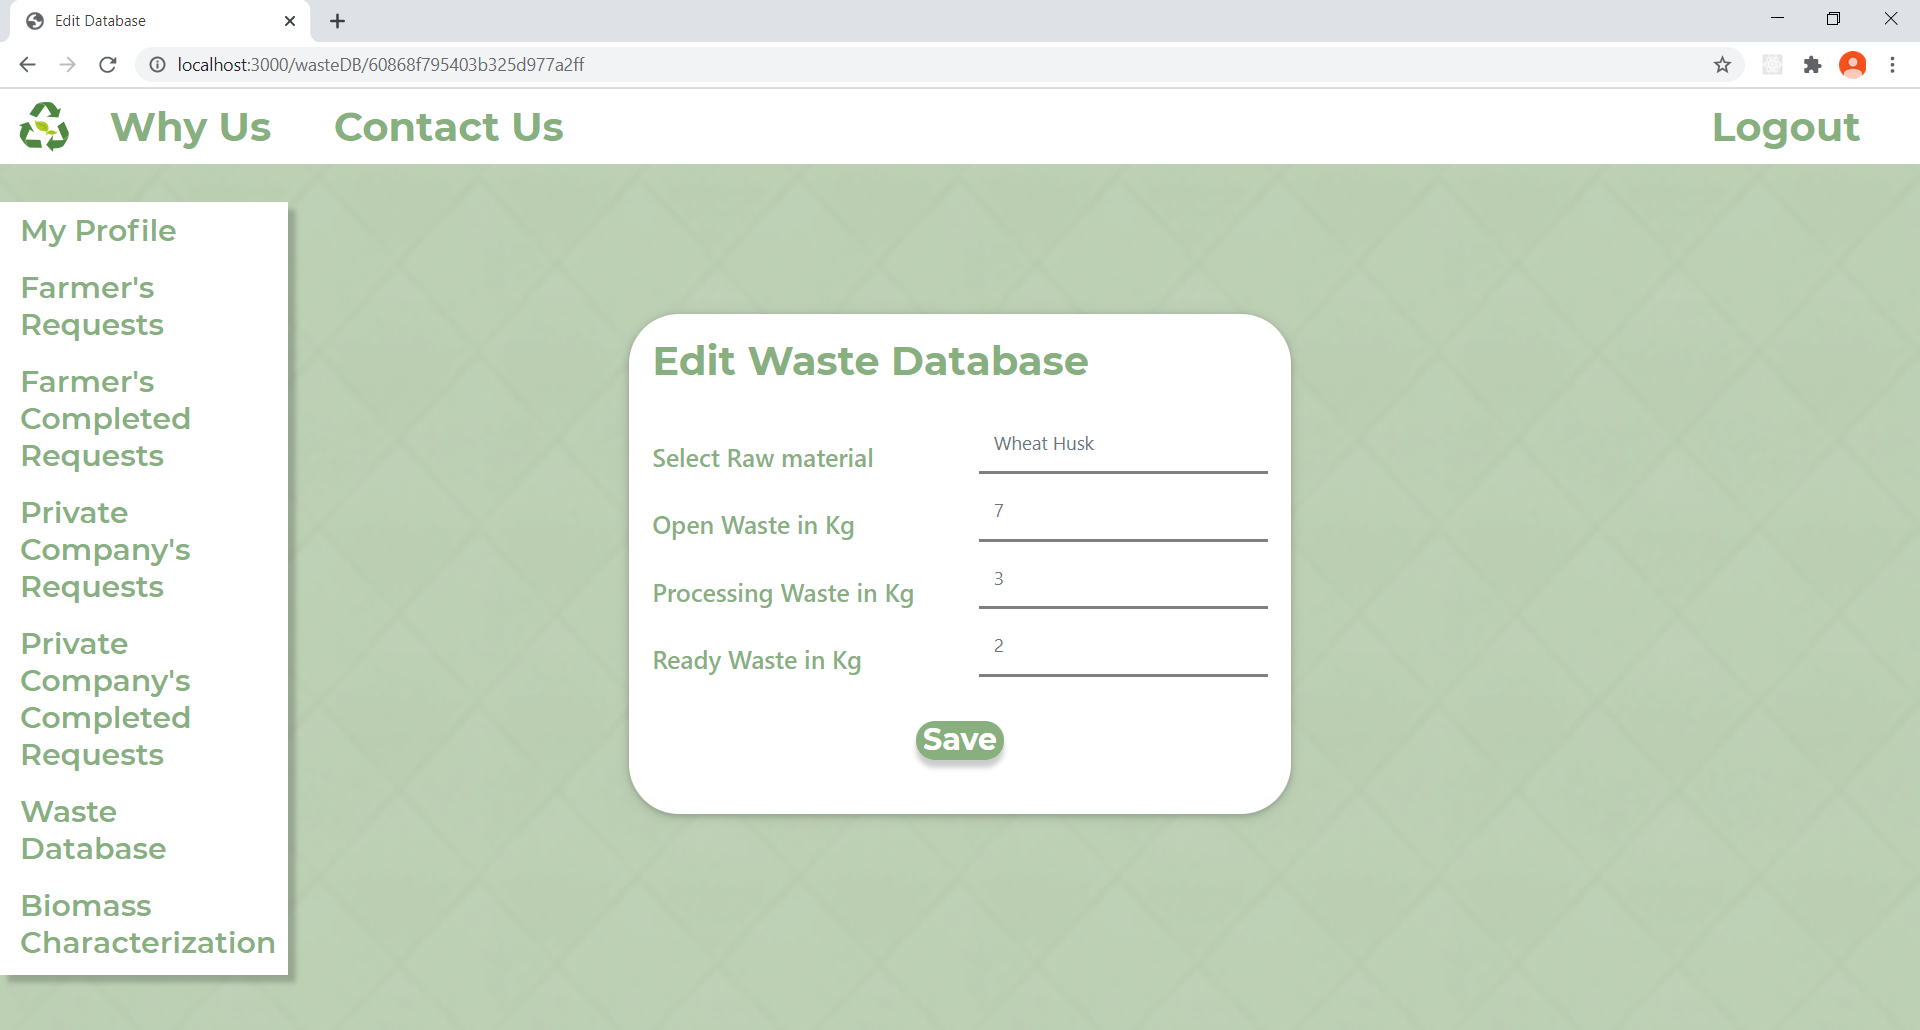
\includegraphics[width=0.5\textwidth,  height=5cm , ,keepaspectratio]{Waste.png}}
         \caption{Edit Waste Database Schema }
         \label{fig:10}
         \end{figure}
\\The maximum value of processing waste can be the waste already in processing + the value of current open waste. So in this example, the maximum value of processing waste can be 10Kg. If the processing waste value is decreased from 3Kg to 2Kg, this leads to an increase in the value of ready waste by 1Kg so now ready waste becomes 3Kg. If the value of processing waste is increased from 3Kg to 6Kg this makes the open waste value decreases by 3Kg and becomes 4Kg.

\subsection{Case: Order By Private Companies}
The figure~\ref{fig:11}  shows that a private company wants to order raw material from the selected collection center. The quantity available at the collection center as shown in the figure~\ref{fig:12} is less than what is specified by the private company then an error will be prompted on the screen "Please visit the raw material Catalogue Page to see the raw material details". Similarly, if the raw material that the private company wants to order is not available then also it shows the same error. If the private company selects the raw material that is present in sufficient quantity at the specified collection center then that order is accepted and is moved to the Pending orders.\\ 
\begin{figure}[htbp]
\centerline{
\includegraphics[width=0.5\textwidth,  height=8cm , ,keepaspectratio]{private.png}}
\caption{Private Company's Add Order Screen }
\label{fig:11}
 \end{figure}
\\For example, if the private company wants to order Cotton Stalk or 3Kg of Wheat Husk refer Figure~\ref{fig:11}, the system will request the private company to choose the raw material present in the raw material catalogue. But if it orders anything less than or equal to 2Kg of Wheat Husk, the order will be placed. \\
         \begin{figure}[htbp]
         \centerline{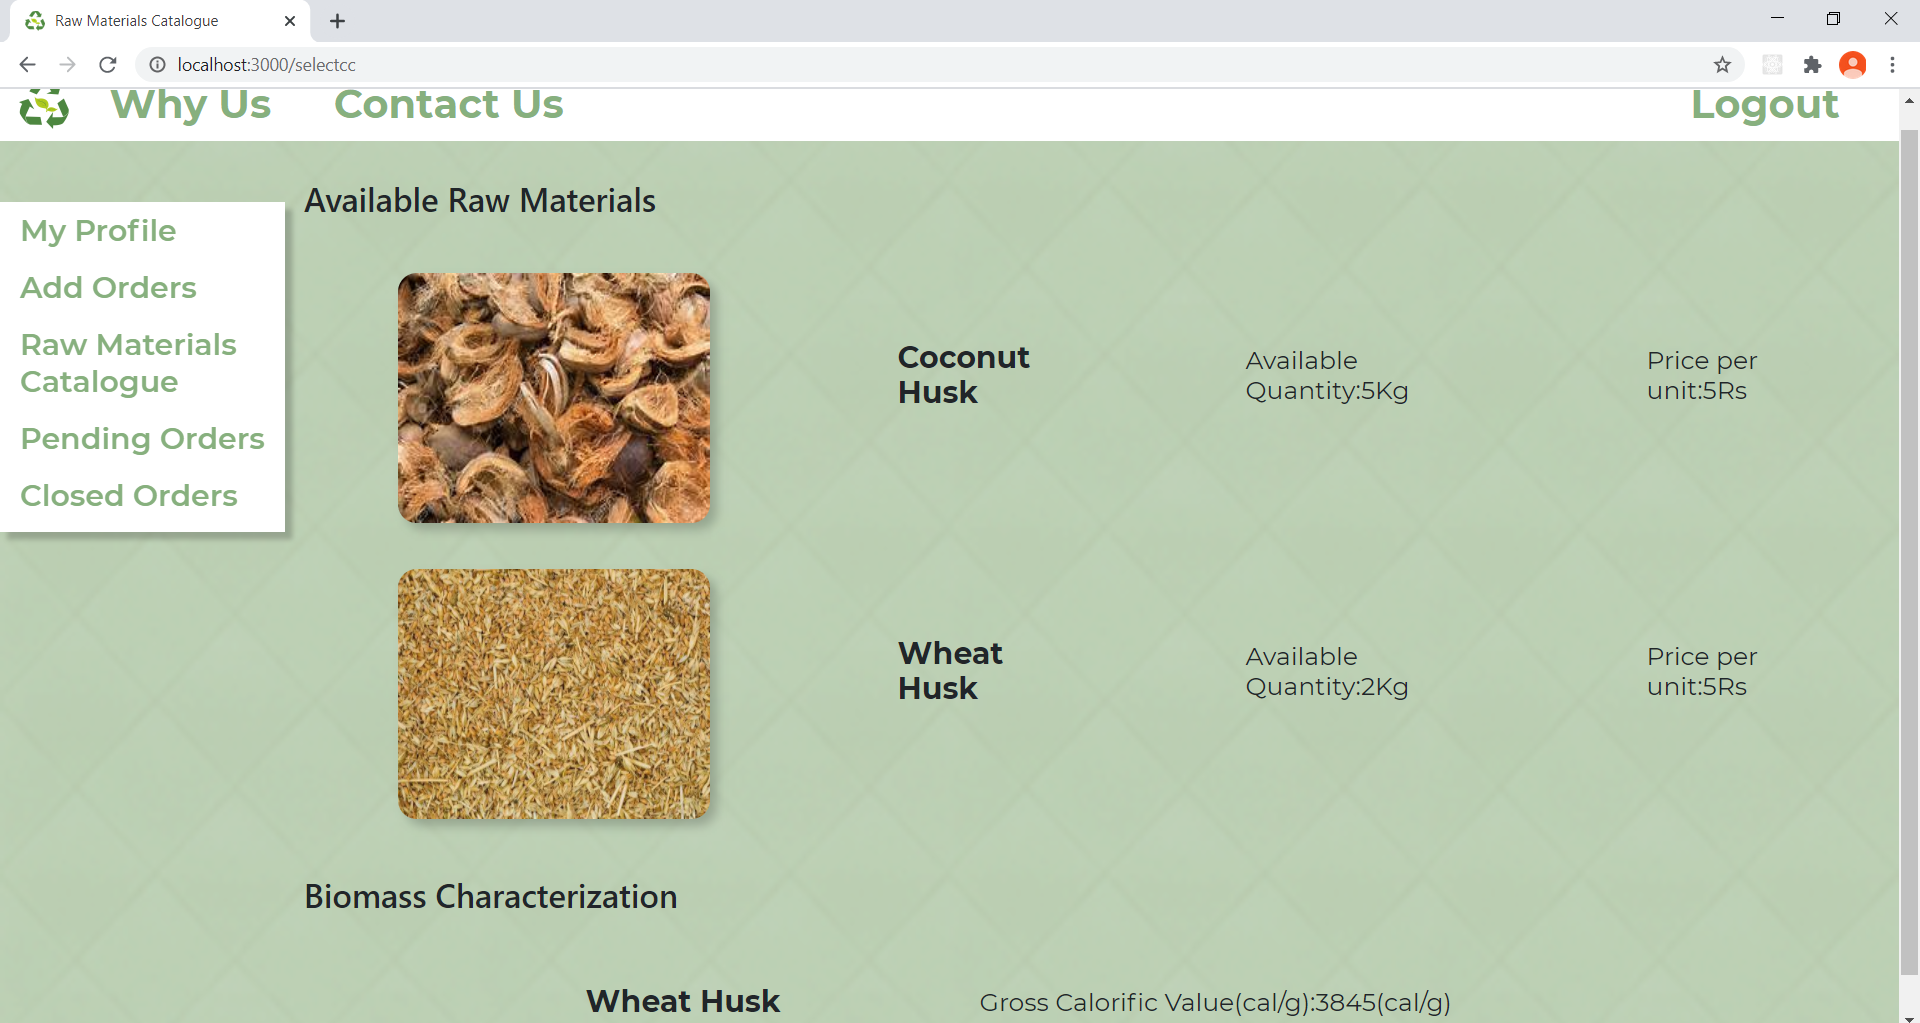
\includegraphics[width=0.5\textwidth,  height=8cm , ,keepaspectratio]{Catalogue.png}}
         \caption{Raw Material Catalogue at the selected Collection Center }
         \label{fig:12}
         \end{figure}
\section{Problems Faced}
\begin{itemize}
    \item To provide authorized access to the stakeholders i.e. the farmer can only view farmer's pages and cannot view private company's, collection center's, and admin's pages the concept of middleware is used which initially we were unaware of.
    \item For the farmer and private company to fill in additional details, a different schema was needed. To achieve this we then used the concept of foreign key and primary key.
    \item To keep the key used to encrypt the password secret, we created a .env file whose content is not visible to everyone.
\end{itemize}

\section{Future Scope}
\begin{itemize}
    \item Our first step will be to translate the website in Hindi and then further to regional languages for easy-of-use for farmers
    \item We would promote digital India and tie-up with banks for creating accounts for farmers, so that all the payment can be digitized
    \item We would like to add the features of GPS order tracking and verification to our model
    \item As mention earlier in section X, we would like to extend the functionality by adding the concept of zamindars who rent out their farms to farmers for growing their crops.  
\end{itemize}

\begin{thebibliography}{00}
\bibitem{b1}Emissions from Crop/Biomass Residue Burning Risk to Atmospheric Quality, International Research Journal Of Earth Sciences - Accepted 4 Februrary 2013 - http://www.isca.in/EARTH\(_\)SCI/Archive/v1/i1/4.ISCA-IRJES-2013-005.pdf
\bibitem{b2}https://abelloncleanenergy.com/
\bibitem{b3} https://nodejs.org/en/
\bibitem{b4} https://expressjs.com/
\bibitem{b5} https://www.w3schools.com/html/default.asp
\bibitem{b6} https://www.w3schools.com/css/default.asp
\bibitem{b7}https://www.javascript.com/
\bibitem{b8} https://www.mongodb.com/
\bibitem{b9}https://ejs.co/
\bibitem{b10}Crop Residue Burning in India: Policy Changes and Potential Solutions, International Journal of Environment Research and Public Health - Published 7 March 2019


\end{thebibliography}

\appendices
\section{Database Schemas} \label{Database Schemas}
\begin{table}[htbp]
\caption{Registeration Schema (Reg Schema)}
\centering
\begin{tabular}{|c|c|c|} 
\hline
\textbf{Field Name} & \textbf{Type}& \textbf{Required / Optional} \\
\hline
Name & String & Required\\
\hline
Add & String & Required\\
\hline
State & String & Required\\
\hline
Contact & String & Required\\
\hline
Username & String & Required\\
\hline
Password & String & Required\\
\hline
Confirm Password & String & Required\\
\hline
Select User Type & String & Required\\
\hline
\end{tabular}
\label{table1}
\begin{center}
Primary Keys: Name , Username
\end{center}
\end{table}
\raggedbottom



\begin{table}[htbp]
\caption{Farmer's Crop Details Schema (FCD Schema)}
\centering
\begin{tabular}{|c|c|c|c|} 
\hline
\textbf{Field Name} & \textbf{Type}& \textbf{Required / Optional} & \textbf{Reference} \\
\hline
Refid & objectId & Required & Table I \\
\hline
Collection Center & String & Required & NULL\\
\hline
Kharif Crops & Array & Required & NULL\\
\hline
Rabi Crops & Array & Required & NULL\\
\hline
\end{tabular}
\label{table3}
\begin{center}
Primary Key: Refid 
\end{center}
\end{table}
\raggedbottom

\begin{table}[htbp]
\caption{Private Companies product Details Schema (PCPD Schema)}
\centering
\begin{tabular}{|c|c|c|c|} 
\hline
\textbf{Field Name} & \textbf{Type}& \textbf{Required / Optional} & \textbf{Reference} \\
\hline
Refid & objectId & Required & Table I \\
\hline
Product & String & Required & NULL\\
\hline
\end{tabular}
\label{table2}
\begin{center}
Primary Key: Refid
\end{center}
\end{table}
\raggedbottom

\begin{table}[htbp]
\caption{Waste Prices Schema (WP Schema)}
\centering
\begin{tabular}{|c|c|c|c|} 
\hline
\textbf{Field Name} & \textbf{Type}& \textbf{Required / Optional}  &\textbf{Reference}\\
\hline
Refid & objectId & Required & Table I\\
\hline
Waste Price & Number & Required & NULL\\
\hline
Raw material Price & Number & Required & NULL\\
\hline
\end{tabular}
\label{table3}
\begin{center}
Primary Key: Refid 
\end{center}
\end{table}
\raggedbottom

\begin{table}[htbp]
\caption{Farmer's Request Details Schema (FRD Schema)}
\centering
\begin{tabular}{|c|c|c|c|} 
\hline
\textbf{Field Name} & \textbf{Type}& \textbf{Required / Optional } & \textbf{Reference} \\
\hline
Refid & objectId & Required & Table I \\
\hline
OrderId & String & Required & NULL \\
\hline
Order Date & String & Required & NULL\\
\hline
Collection Center & String & Required & Table II\\
\hline
Raw Material & String & Required & NULL\\
\hline
Land Area & Number & Required & NULL\\
\hline
Harvesting Date & String & Required & NULL\\
\hline
Approved Request & Boolean & Optional & NULL\\
\hline
Pickup Date & String & Optional & NULL\\
\hline
In transit & Boolean & Optional & NULL\\
\hline
Ready & Boolean & Optional & NULL\\
\hline
Paid & Boolean & Optional & NULL\\
\hline
Waste Amount & Number & Optional & NULL\\
\hline
Payment Amount & Number & Optional & NULL\\
\hline
Order Close Date & String & Optional & NULL\\
\hline
Year & String & Optional & NULL\\
\hline
\end{tabular}
\label{table4}
\begin{center}
Primary Keys: Refid , OrderId
\end{center}
\end{table}
\raggedbottom

\begin{table}[htbp]
\caption{Waste Details Schema (WD Schema)}
\centering
\begin{tabular}{|c|c|c|c|} 
\hline
\textbf{Field Name} & \textbf{Type}& \textbf{Required / Optional} & \textbf{Reference} \\
\hline
Refid & objectId & Required & Table I \\
\hline
Raw Material & String & Required & NULL \\
\hline
Open Waste & Number & Required & NULL\\
\hline
Processing Waste & Number & Required & NULL\\
\hline
Ready Waste & Number & Required & NULL\\
\hline
\end{tabular}
\label{table5}
\begin{center}
Primary Key: [Refid , Raw Material]
\end{center}
\end{table}
\raggedbottom

\begin{table}[htbp]
\caption{Biomass Characterization Details Schema (BCD Schema)}
\centering
\begin{tabular}{|c|c|c|c|} 
\hline
\textbf{Field Name} & \textbf{Type}& \textbf{Required / Optional} & \textbf{Reference} \\
\hline
Refid & objectId & Required & Table I \\
\hline
Raw Material & String & Required & NULL \\
\hline
Gross Calorific Value & Number & Required & NULL\\
\hline
\end{tabular}
\label{table6}
\begin{center}
Primary Key: [Refid , Raw Material]
\end{center}
\end{table}
\raggedbottom

\begin{table}[htbp]
\caption{Private Companies Order Details Schema (PCOD Schema)}
\centering
\begin{tabular}{|c|c|c|c|} 
\hline
\textbf{Field Name} & \textbf{Type}& \textbf{Required / Optional } & \textbf{Reference} \\
\hline
Refid & objectId & Required & Table I \\
\hline
OrderId & String & Required & NULL \\
\hline
Product & String & Required & Table III \\
\hline
Order Date & String & Required & NULL\\
\hline
Collection Center & String & Required & NULL\\
\hline
Raw Material  & String & Required & NULL\\
\hline
Quantity & Number & Required & NULL\\
\hline
Pickup Date & String & Required & NULL\\
\hline
Approve & Boolean & Optional & NULL\\
\hline
Paid & Boolean & Optional & NULL\\
\hline
Payment Amount & Number & Optional & NULL\\
\hline
\end{tabular}
\label{table7}
\begin{center}
Primary Keys: Refid , OrderId
\end{center}
\end{table}
\raggedbottom
\hfill \break
\section{Abbreviations} \label{Abbreviations}
\begin{itemize}
    \item KAPS: Krishi Avashesh Prabandhan Seva
    \item HTML: Hyper Text markup Language
    \item CSS : Cascading Style Sheets
    \item Reg: Registration 
    \item FCD: Farmer's Crop Details 
    \item PCPD: Private Company's Product Details 
    \item WP: Waste Prices 
    \item FRD: Farmer's Request Details 
    \item WD: Waste Details 
    \item BCD: Biomass Characterization Details 
    \item PCOD: Private Company Order Details 
    \item Mt: Million Ton
\end{itemize}


\end{document}
